\documentclass{standalone}
\usepackage{tikz}
\usetikzlibrary{arrows}
\usetikzlibrary{shapes.multipart}
\usetikzlibrary{shapes,snakes}
\usepackage[bitstream-charter]{mathdesign}

\newcommand\irregularcircle[2]{% radius, irregularity
\pgfextra {\pgfmathsetmacro\len{(#1)+rand*(#2)}}
+(0:\len pt)
\foreach \a in {10,20,...,350}{
  \pgfextra {\pgfmathsetmacro\len{(#1)+rand*(#2)}}
  -- +(\a:\len pt)
} -- cycle
}



\begin{document}
  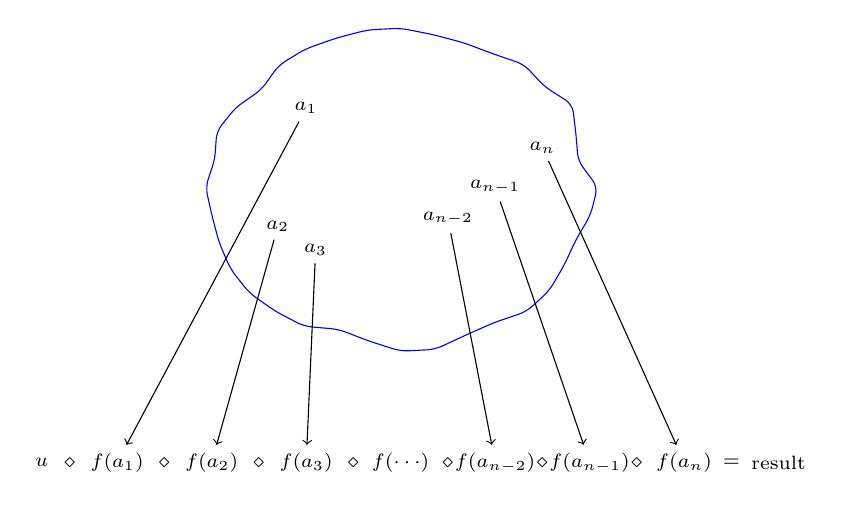
\begin{tikzpicture}[xscale=1.2]
    \scriptsize
    \coordinate (c) at (3.5,2);
    \draw[blue,rounded corners=1mm] (c) \irregularcircle{2cm}{1mm};

    \foreach \x/\t/\k/\y in 
       {2.5/$a_1$/0/3,2.2/$a_2$/1/1.5,2.6/$a_3$/2/1.2,4/$a_{n-2}$/4/1.6,4.5/$a_{n-1}$/5/2,5/$a_n$/6/2.5} 
        \node (a\k) at (\x,\y) {\t};
    \foreach \x/\t/\k in {.5/$a_1$/0,1.5/$a_2$/1,2.5/$a_3$/2,3.5/$\cdots$/3,4.5/$a_{n-2}$/4,5.5/$a_{n-1}$/5,6.5/$a_n$/6} {
            \node (f\k) at (\x,-1.5) {$f($\t$)$};
    }
    \foreach \k in {0,1,2}
      \draw[->] (a\k) -- (f\k);
    \foreach \k in {4,5,6}
      \draw[->] (a\k) -- (f\k);

    \foreach \x in {0,1,2,3,4,5,6}
      \node at (\x,-1.5) {$\diamond$};

    \node at (7,-1.5) {$=$}; 
    \node at (7.5,-1.5) {result};
    \node at (-0.3,-1.5) {$u$};
\end{tikzpicture}
\end{document}


